%
% File: chap04.tex
% Author: Nadeem Gul Rintu Daniel
% Description: Gives an Overview of the Geographic Coordinate System and the coordinate System which is implemented within the Floe Navigation System
%
\let\textcircled=\pgftextcircled
\chapter{System Overview}
\label{chap:systemoverview}
\noindent
\initial{T}his section gives an overview of the Geographic Coordinate System. It will briefly introduce the concept of geographic coordinates and the Global Positioning System and how physical locations are mapped to coordinates on a 2D plane. It also gives a detailed description of the custom coordinate system, which is derived from the Global Coordinate System, that is implemented as part of the Floe Navigation System.
\section{Geographic Coordinate System}
The purpose of any coordinate system is to specify a location on a 
\section{Mapping}
\label{sec:sec4_2}
\noindent
%
The Floe Navigation System projects the Geographic coordinate system on to a $2$D plane with Latitude along the y-axis and Longitude along the x-axis. The intersection of the prime meridian and the equator (\ang{0}, \ang{0}) is the origin of the $2$D plane. The mapping is done in such a fashion that \ang{1} along the latitude axis represents $60$ Nautical Miles. Since the Earth is not a perfect sphere and longitudinal lines are closer together at poles and farther apart near the equator so \ang{1} along the longitude axis represents \SI{60}{\nauticalmile} at the equator and as we move towards the poles the distance represented by \ang{1} decreases by a factor cosine of the latitude. So, on the longitude axis, \ang{1} represents $\SI{60}{\nauticalmile} \times \cos(latitude)$.
\begin{figure}[h]
	\centering
	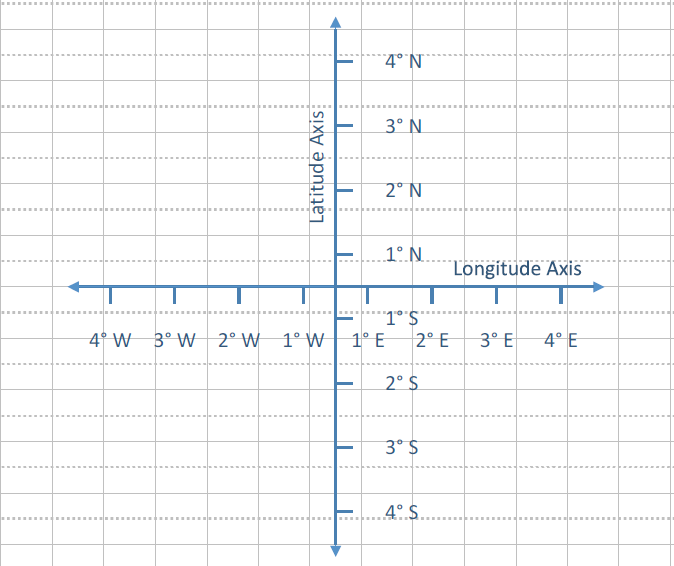
\includegraphics[height=0.45\textheight]{fig04/2DProject}
	\mycaption[Map Projection.]{Map Projection.}
	\label{fig:CH4MapProjection}
\end{figure}
%
\section{Custom Coordinate System}
\label{sec:sec4_3}
\noindent
%
The Custom Coordinate System is a Cartesian Coordinate System established on the Ice Floe. As with any Cartesian Coordinate System, each point is expressed as an ordered pair. The elements of the ordered pair represent the distance measured from an axis. The first element of the ordered pair is the distance from the x-axis and is called the x-coordinate and second element of the ordered pair is the distance from y-axis and is called the y-coordinate~\cite{van2010basic}. The Custom Coordinate System within the Geographic Coordinate System is shown in Figure~\ref{fig:CH4CustomCoordinate}
\begin{figure}[h]
	\centering
	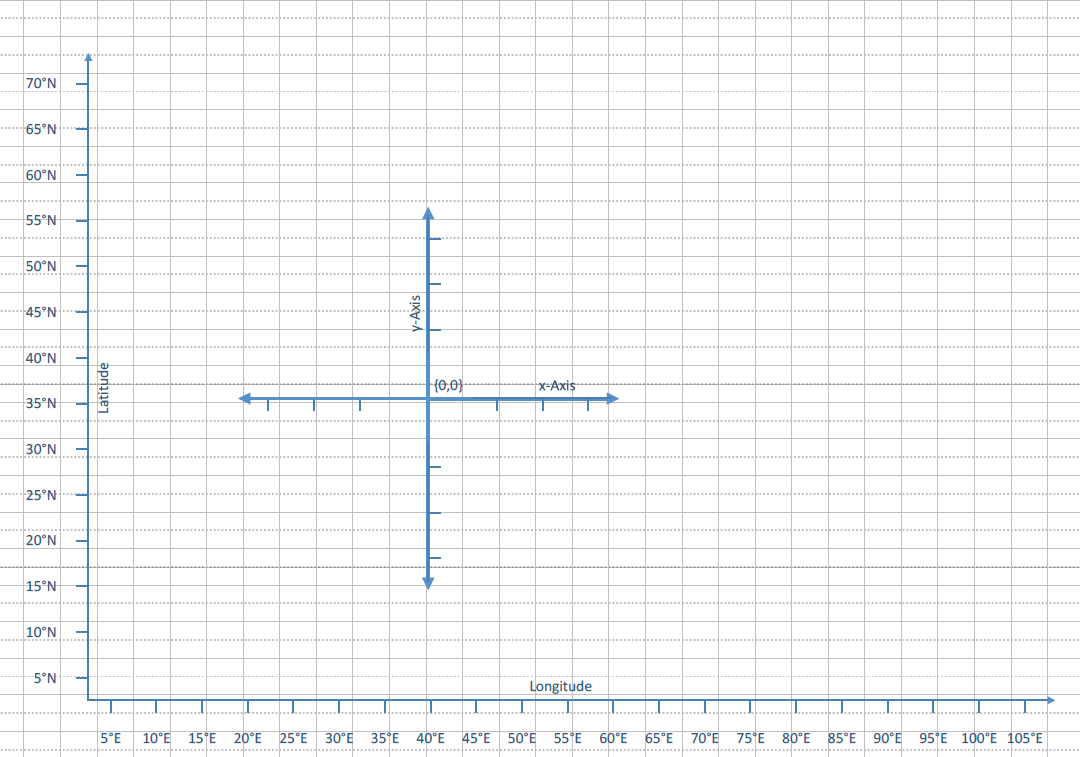
\includegraphics[height=0.45\textheight]{fig04/cartesiancoordinates.png}
	\mycaption[Custom Coordinate System within Geographic Coordinate System.]{Custom Coordinate System within Geographic Coordinate System.}
	\label{fig:CH4CustomCoordinate}
\end{figure}
%
\newline
\noindent
The Floe Navigation System needs at least two AIS transponders to create the coordinate system which is formed by designating one AIS transponder as an origin of the coordinate system (called the Origin Station) and another AIS transponder is used to mark the direction of the x-axis (called the x-Axis Marker). The y-axis of the coordinate system is considered perpendicular to the x-axis. The AIS transponder moves with Sea Ice and broadcast their geographical coordinates periodically with the movement. As the Geographical coordinates are updated, the system recalculates the coordinate system and the position of all the objects (stations and other points of interest) marked on the coordinate system along with it. 
%
\subsection{Angle Beta}
\label{subsec:subsec4_3_1}
\noindent
The mapping from the Geographic coordinates to the custom coordinate system is done by calculating the angle between the x-Axis (marked by the two AIS transponders: Origin Station and x-Axis Marker) of the custom coordinate system and the Geographic Longitudinal direction. The angle of the custom coordinate system's x-Axis to the Geographic Longitudinal axis is called Beta angle denoted by $\beta$ as shown in figure~\ref{fig:CH4CoordinateSystemDef}
\begin{figure}[h]
	\centering
	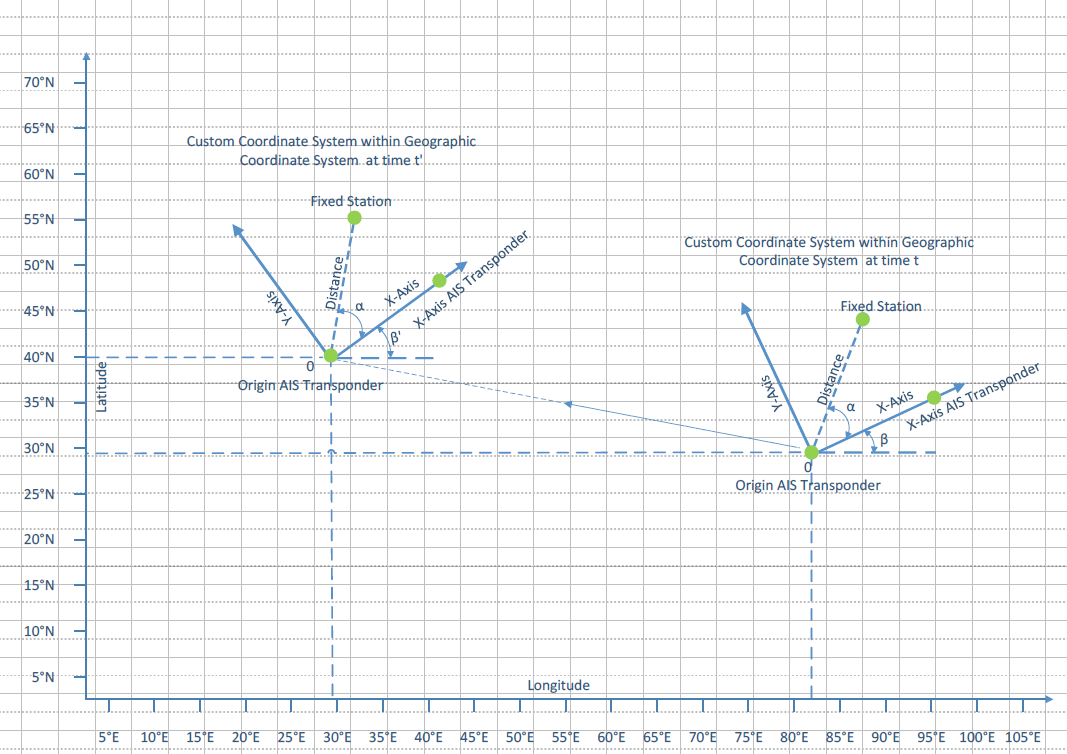
\includegraphics[height=0.45\textheight]{fig04/AngleBetaDef.png}
	\mycaption[Custom Coordinate System with Angle Beta.]{Custom Coordinate System with Angle Beta.}
	\label{fig:CH4CoordinateSystemDef}
\end{figure} 
\newline
\noindent
The angle $\beta$ is calculated by calculating the initial bearing angle from the Origin Station to the x-Axis Marker using the Haversine formula. The Haversine formula is a method of computing the great-circle distance between two points on a sphere given their latitude and longitude. It is derived from the spherical law of cosines~\cite{haversineDef}. According to the Haversine formula given the latitude and longitude of two points the initial bearing is given by~\ref{eq:bearing}~\cite{haversineBear}
	\begin{equation} \label{eq:bearing}
		\theta = \taninv\frac{\sin(\Delta\lambda)\cdot\cos(\phi_{2})}{\cos(\phi_{1})\cdot\sin(\phi_{2}) - \sin(\phi_{1})\cdot\cos(\phi_{2})\cdot\cos(\Delta\lambda)}
		\tag{4.1}		
	\end{equation}
where:
	\begin{conditions}
		\theta	&		Bearing \\
		\phi_{1}	&		Latitude of First Point \\
		\lambda_{1}	&	Longitude of First Point \\
		\phi_{2}	&	Latitude of Second Point \\
		\lambda_{2}	&	Longitude of Second Point \\
		\Delta\lambda	&	Difference in Longitude \\
	\end{conditions}
\newline
\noindent
Angle $\beta$ is used for the calculation of coordinates in the Grid and it is of paramount importance for the calculation of the coordinates of other points on the Floe.
%
\subsection{Angle Theta}
\label{subsec:subsec4_3_2}
\noindent

Every new Fixed Station (mounted with an AIS Transponder) that is installed is specified by its distance from the origin and the angle $\alpha$ it makes with the x-Axis of the custom coordinate system. A simplified version of this scenario is shown in Figure 2.3. The angle $\alpha$ and the distance for all Fixed Station are considered to be constant\footnotemark[1] and the angle $\beta$ can be recalculated from the constant $\alpha$ and distance from each Fixed Station.
\footnotetext[1]{This distance may change with the Expansion/Shear of the Floe. However, for simplification purposes, the distance is assumed constant.}
\newline
\noindent 
The value of angle $\beta$ is updated at regular time intervals (\SI{10}{\second}) by calculating a new value from the location data received from each Fixed Stations and averaging it; so that if any of the Fixed Stations (including the origin and x-Axis marker) breaks away from the Ice, it does not affect the value of $\beta$ greatly and the coordinate system persists. So, the coordinate system is independent of the Fixed Stations; as long as there are two Fixed Stations installed the system can function.
\newline
\noindent 
AIS Transponders which are not installed as Fixed Station are shown as Mobile Stations and for each of these mobile stations, the app calculates the angle $\alpha$ and distance at regular time intervals from the location data received from the AIS Transponder.
\newline
\noindent
There are certain points on the Sea Ice which do not have an AIS Station mounted such as Static Stations or Waypoints. For these points, the system calculates the angle $\alpha$ and distance from origin using the tablet’s location at the time of installation. As these points are considered to be stationary on the Ice, these parameters are not recalculated again and it remains constant unless the point is recovered. 
